\documentclass[11pt,a4paper]{book}
\usepackage[english,greek]{babel}
\usepackage[utf8x]{inputenc}
\usepackage{amssymb,latexsym,amsmath,ucs,amsthm,setspace,graphicx}
\usepackage{kerkis}
\newtheorem*{lemma}{Λήμμα}
\newcommand{\HRule}{\rule{\linewidth}{0.5mm}}
\newcommand{\defeq}{\overset{\underset{\mathrm{def}}{}}{=}}
\makeatletter
\def\imod#1{\allowbreak\mkern10mu({\operator@font mod}\,\,#1)}
\makeatother
\raggedbottom
\begin{document}

\begin{titlepage}
\begin{center}

\includegraphics[width=0.15\textwidth]{Pyrforos2.png}\\[1.cm]
\textsc{\LARGE Εθνικό Μετσόβιο Πολυτεχνείο}\\[1.5cm]

\Large{ Σημειώσεις Διαλέξεων }\\[0.5cm]

% Title
\begin{doublespace}
\HRule \\[0.4cm]
{\huge \bfseries
Στοιχεία Θεωρίας Αριθμών
\\
\&
\\
Εφαρμογές στην Κρυπτογραφία
}\\[0.4cm]
\end{doublespace}

\HRule \\[1.5cm]

\begin{minipage}{0.4\textwidth}
\begin{flushleft} \large
\emph{Επιμέλεια σημειώσεων:}\\
Διονύσης \textsc{Ζήνδρος}
Αντώνης \textsc{Αναστασόπουλος}
\end{flushleft}
\end{minipage}
\begin{minipage}{0.4\textwidth}
\begin{flushright} \large
\emph{Διδάσκοντες:} \\
Στάθης \textsc{Ζάχος}\\
Άρης \textsc{Παγουρτζής}
\end{flushright}
\end{minipage}

\vfill

{\large 28 Νοεμβρίου 2011}
\end{center}
\end{titlepage}

\section*{Θεωρία αριθμών}

Από τις σημειώσεις [Ζάχος]: Κεφάλαιο 6, σελίδα 145.

\subsection*{Διαιρετότητα}

\[
a|b \defeq  \exists c \in \mathbb{Z}: b = ca
\]

\subsection*{Ιδιότητες}

\begin{enumerate}
	\item $ a | 0 $
	\item Κάθε αριθμός μεγαλύτερος του 1 έχει τουλάχιστον δύο διαιρέτες: το 1 και τον εαυτό του
	\item $ a|b \Rightarrow a | (bc) $
	\item $ a|b \land b|a \Rightarrow a|c $
	\item $ a|b \land b|a \Leftrightarrow |a| = |b| $
	\item $ a|b \land a|c \Rightarrow a | ( b + c ) $
	\item $ a|b \land a|c \Rightarrow a | (bx + cy) $
	\item $ a|b \land b>0 \Rightarrow a \leq b$
\end{enumerate}

\subsection*{Πρώτος αριθμός}

\[
a \in \mathbb{N} \text{ πρώτος} \defeq \forall b \in \mathbb{N}: 1 < b < a \Rightarrow b \nmid a
\]

\subsection*{Γνωστοί πρώτοι}
\begin{enumerate}
	\item $2, 3, 5, ..., 1997, 1999, 2003, 2011, ...$
	\item Ο μεγαλύτερος γνωστός πρώτος το 2011: $2^{43112609} - 1$ [\latintext{GIMPS}]
\end{enumerate}

\subsection*{Σχετικά πρώτοι}

\[
a \textlatin{ coprime } b \defeq gcd( a, b ) = 1
\]

\subsection*{Μέγιστος Κοινός Διαιρέτης}

\begin{align*}
	( a, b ) &\defeq\\
	gcd( a, b ) &\defeq \max\{ c \in \mathbb{Z}: c|a \land c|b \}
\end{align*}

Ο καλύτερος αλγόριθμος που γνωρίζουμε ακόμα και σήμερα για την εύρεσή του είναι ο αλγόριθμος του Ευκλείδη:

\begin{itemize}
	\item $ gcd( a, b ) = b $, αν $ b|a $ και $ a > b $
	\item $ gcd( a, b ) = gcd( a \mod b, b ) $, αν $ b \nmid a $ και $ a > b $
	\item $ gcd( a, b ) = gcd( b, a ) $, αλλιώς
\end{itemize}

\section*{Αλγεβρικές δομές}

\subsection*{Ομάδες}

\textlatin{Abelian group} ή αντιμεταθετική ομάδα λέγεται ένα ζεύγος $(G, *)$ τέτοιο ώστε για $a, b, c \in G$:

\begin{itemize}
	\item $a * (b * c) = (a * b) * c$
	\item $a * b = b  * a$
	\item $\exists! e \in G: \forall a: a * e = a$
	\item $ \forall a \in a^{-1} \in G: a * a^{-1} = e$
\end{itemize}

\subsection*{Αλγεβρική δομή}
Αλγεβρική δομή λέγεται μία \textlatin{n-}άδα $( A; f_1, f_2, f_3, \ldots )$
όπου $A$ ένα σύνολο (\textlatin{domain}) και $f_1, f_2, f_3, \ldots$ πράξεις
(δηλαδή συναρτήσεις κλειστές εντός του $A$) με 0 ή περισσότερα ορίσματα με πεδίο ορισμού το $A$.

\subsection*{Ομομορφισμός}
Mία συνάρτηση $f: A \rightarrow B$ ανάμεσα σε δύο αλγεβρικές δομές $(A, \oplus)$ και $(B, \otimes)$ ονομάζεται ομομορφισμός αν απεικονίζει τη μία αλγεβρική δομή στην άλλη ως εξής:

\[
	f( a \oplus b ) = f( a ) \otimes f( b )
\]
\begin{align*}
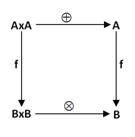
\includegraphics[width=0.4\textwidth]{comm-diagram.png}\\[1.cm]
\end{align*}

Από τον ορισμό προκύπτει άμεσα ότι:

\begin{align*}
    f( e_A \oplus b ) &= f( e_A ) \otimes f( b )\\
	f( b ) &= e_B \otimes f( b )\\
	f( e_A ) &= e_B
\end{align*}

\subsection*{Δακτύλιος}

\begin{align*}
(R, +, *) \text{ δακτύλιος} &\defeq\\
(R, +) &\text{ αντιμεταθετική ομάδα}\\
\land \forall a, b, c &\in R:\\
a * (b + c ) &= (a * b + a * c)\\
\land (b + c) * a &= b * a + c * a
\end{align*}

\subsection*{Σώμα}
\begin{align*}
(F, +, *) \text{ σώμα } &\defeq\\
&(F, +) \text{ αντιμεταθετική ομάδα }\\
\land &(F - \{e_+\}, *) \text{ αντιμεταθετική ομάδα }\\
\land &\forall a, b, c \in F: a * (b + c) = a * b + a * c
\end{align*}

\subsection*{Υποομάδα}
\begin{align*}
 (S, *) \text{ υποομάδα της } (G, *) &\defeq S \subseteq G \land (S, *) \text{ ομάδα}
\end{align*}

\subsection*{Κυκλική ομάδα}
\[
	( G, * ) \text{ κυκλική} \defeq \exists g \in (G, *): \forall x \in G: \exists y \in \mathbb{N}: x = g^y
\]

\subsection*{Τάξη}
\begin{align*}
	a^1 &\defeq a\\
	a^n &\defeq a^{n - 1} * a\\
	\text{ τάξη } a &\defeq min\{ y \in \mathbb{N}: a^y = e \}
\end{align*}

\subsection*{Γεννήτορας}
\[
	a \text{ γεννήτορας της } G \defeq \text{τάξη } a = |G|
\]

\subsection*{\textlatin{Coset}}
\[
H * a =\{h * a : h \in H, a \in G\} \defeq \text{ δεξί σύμπλοκο (\textlatin{coset}) της } H \text { στη } G 
\]
\[
\text { για } Η \text{ υποoμάδα της } (G,*).
\]
\begin{align*}
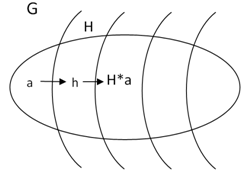
\includegraphics[width=0.6\textwidth]{baseBall.png}\\[1.cm]
\end{align*}

\subsection*{\textlatin{Quotient group}}
\[
\text {Το σύνολο }\{G/H\} \text{ είναι ομάδα με πράξη } (H*a)*(H*b)=H*(a*b).
\]

\subsection*{\textlatin{Lagrange}}
\[
\text {Αν }H \text{ υποομάδα της πεπερασμένης ομάδας } G \text{ τότε}\]
\[|G|=|G/H|*|H|
\]
\section*{Ο δακτύλιος $\mathbb{Z}_m$}
\[
\text{Το σύνολο ακεραίων } \textlatin{modulo m : } \{0,1,2,...,m-1\}.
\]
\[\text{Ισοδύναμα } \mathbb{Z}_m = \{a \mod m | a\in \mathbb{Z}\}\]
\subsection*{Υπόλοιπο}

\begin{align*}
	a \equiv_m b &\defeq \\
	a \equiv b \imod m &\defeq m | ( a - b )
\end{align*}

\subsection*{Ιδιότητες υπολοίπου}

\begin{enumerate}
	\item $a \equiv a \imod m$ (\textlatin{reflexive})
	\item $a \equiv b \imod m \Rightarrow b \equiv a \imod m$ (\textlatin{symmetric})
	\item $a \equiv b \imod m \land b \equiv c \imod n \Rightarrow a \equiv c \imod m$ (\textlatin{transitive})
\end{enumerate}

\subsection*{Ιδιότητες κλάσεων}
\begin{enumerate}
	\item $[a] + [b] = [a + b]$
	\item $[a].[b] = [a.b]$
	\item $[a] + [b] = [b] + [a]$
	\item $([a] + [b]) + [c] = [a] + ([b] + [c])$
	\item $[a] + [0] = [a]$
	\item $[a] + [-a] = [0]$
	\item $[a].[b] = [b].[a]$
	\item $([a].[b]).[c] = [a].([b].[c])$
	\item $[a].([b]+[c]) = [a].[b] + [a].[c]$
	\item $[a].[1] = [a]$
\end{enumerate}

\subsection*{Ασκήσεις}
\begin{enumerate}
	\item Να αποδείξετε την Πρόταση 6.2, [Ζάχος] σ. 146
	\item Άσκηση 6.8, [Ζάχος] σ. 147
	\item Να αποδείξετε την ορθότητα του αλγορίθμου του Ευκλείδη, [Ζάχος] σ. 148
	\item Να αποδείξετε την Πρόταση 6.15, [Ζάχος] σ. 149
	\item Να αποδείξετε το Πόρισμα 6.17, [Ζάχος] σ. 149
	\item Να αποδείξετε το Θεώρημα 6.19, [Ζάχος] σ. 149
	\item Άσκηση 6.37, [Ζάχος] σ. 154
	\item Άσκηση 6.40, [Ζάχος] σ. 155
\end{enumerate}

\section*{Βιβλιογραφία}
\begin{enumerate}
	\item \text{[}Ζάχος\text{]}: Ε. Ζάχος, ((Σημειώσεις στη Θεωρία Αριθμων και την Κρυπτογραφία)), 2007
	\item \text{[}\textlatin{GIMPS}\text{]}:: ((\textlatin{Great Internet Mersenne Prime Search})), 1996 - 2011
\end{enumerate}
\end{document}
